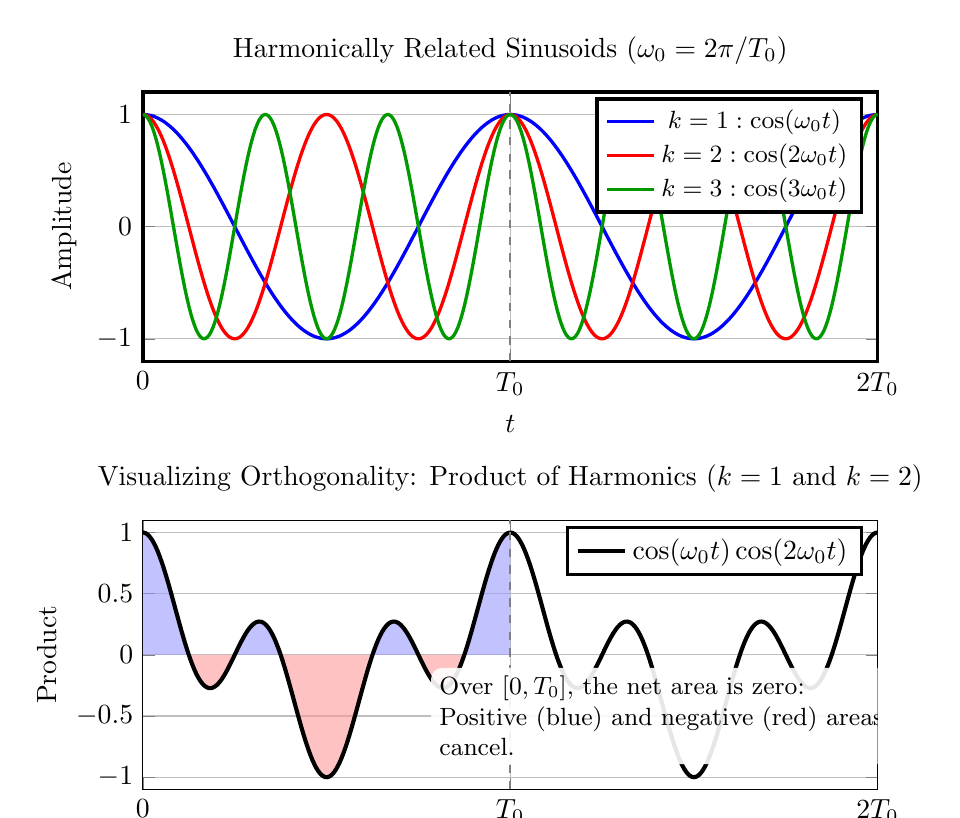
\begin{tikzpicture}
	\usepgfplotslibrary{fillbetween}
	
	% --- TOP PLOT: The Harmonics ---
	\begin{axis}[
		name=plot_harmonics,
		width=0.9\textwidth,
		height=5cm,
		title={Harmonically Related Sinusoids ($\omega_0 = 2\pi/T_0$)},
		xlabel={\(t\)},
		ylabel={Amplitude},
		grid=major,
		xmin=0, xmax=2,
		ymin=-1.2, ymax=1.2,
		xtick={0, 1, 2},
		xticklabels={\(0\), \(T_0\), \(2T_0\)},
		ytick={-1, 0, 1},
		legend style={at={(0.98,0.98)}, anchor=north east, font=\small},
		trig format plots=rad,
		samples=400,
		thick,
		no marks,
		line width=1.2pt,
		]
		% k=1 (Fundamental)
		\addplot[blue, domain=0:2] {cos(2*pi*x)};
		\addlegendentry{\(k=1: \cos(\omega_0 t)\)}
		
		% k=2
		\addplot[red, domain=0:2] {cos(4*pi*x)};
		\addlegendentry{\(k=2: \cos(2\omega_0 t)\)}
		
		% k=3
		\addplot[green!60!black, domain=0:2] {cos(6*pi*x)};
		\addlegendentry{\(k=3: \cos(3\omega_0 t)\)}
		
		% Period marker
		\draw[dashed, gray, thick] (axis cs:1,-1.2) -- (axis cs:1,1.2);
		\node[anchor=south, font=\footnotesize] at (axis cs:1,1.2) {\(T_0\)};
	\end{axis}
	
	% --- BOTTOM PLOT: Demonstrating Orthogonality ---
	\begin{axis}[
		at={(plot_harmonics.below south)},
		anchor=north,
		yshift=-1cm,
		width=0.9\textwidth,
		height=5cm,
		title={Visualizing Orthogonality: Product of Harmonics (\(k=1\) and \(k=2\))},
		xlabel={\(t\)},
		ylabel={Product},
		grid=major,
		xmin=0, xmax=2,
		ymin=-1.1, ymax=1.1,
		xtick={0, 1, 2},
		xticklabels={\(0\), \(T_0\), \(2T_0\)},
		ytick={-1, -0.5, 0, 0.5, 1},
		trig format plots=rad,
		samples=400,
		thick,
		no marks,
		line width=1.2pt,
		]
		% Plot the product of the first two harmonics
		\addplot[name path=product, domain=0:2, black, line width=1.5pt] 
		{cos(2*pi*x) * cos(4*pi*x)};
		\addlegendentry{\(\cos(\omega_0 t)\cos(2\omega_0 t)\)}
		
		% Path for the x-axis (to fill between)
		\path[name path=xaxis] (axis cs:0,0) -- (axis cs:2,0);
		
		% Fill the area between the product curve and x-axis over [0, T_0]
		\addplot[draw=none] fill between[
		of=product and xaxis,
		soft clip={domain=0:1},
		split,
		every even segment/.style={fill=blue!40, opacity=0.6},
		every odd segment/.style={fill=red!40, opacity=0.6},
		];
		
		% Period marker
		\draw[dashed, gray, thick] (axis cs:1,-1.1) -- (axis cs:1,1.1);
		\node[anchor=south, font=\footnotesize] at (axis cs:1,1.1) {\(T_0\)};
		
		% Annotation explaining the concept
		\node[align=left, text width=6cm, font=\small, fill=white, fill opacity=0.9, 
		text opacity=1, rounded corners, inner sep=3pt] at (axis cs:1.45, -0.5) {
			Over \([0, T_0]\), the net area is zero:\\
			Positive (blue) and negative (red) areas cancel.
		};
	\end{axis}
	
\end{tikzpicture}
